
\chapter{Eksamen}
\href{https://sokeresultat.udir.no/eksamensoppgaver.html?query=AUT4002}{Samle side for eksamensoppgaver}


\section{Typiske eksamensoppgaver}

Her er det samlet en oversikt over typiske oppgaver som kommer på en eksamen. Det er ment å være til hjelp når en  øver seg på  å løse eksamensoppgaver og under forberedelsesdagene. Det er viktig å være klar over at eksamen har en tendens til å forandre seg for hvert år. En må derfor regne med at det kommer oppaver som ikke er beskrevet her. Har du kontroll på de oppgavene som er beskrevet her har du hvertfall et godt utgangpunkt før eksamen. 

\subsection{Sjekk vedlikehold av transmitter}

I denne type oppgaver kan komme i ulike versjoner, men som regel går det ut på å ta seg ut i anlegg og sjekke kalibre en transmitter. 
\subsubsection*{Planlegging}
Lag en fredriftsplan som inneholder de ulike deloppgavene  som jobben inneholder. 
F.eks. 
\begin{itemize}
	\item ta på verneutstyr
	\item sjekke transmitter for skader o.l. 
	\item frakobling av transmitter
	\item kalibrering
	\item tilbakestilling/rydding
	\item dokumentasjon
\end{itemize}


Tenk igjennom deloppgavene fra fremdriftsplanen og vurder risiko og eventuelle tiltak. Typiske ting en kan være obs på er:
\begin{itemize}
	\item hva er vanlig verneutstyr ute i anlegget på bedriften.
	\item Du bør tenke på hvordan transmitteren kobles fra prosessen og hvilke konsekvenser dette får. Er det Block \& bleed ventil? 
	\item Er det aktuelt med andre som jobber i nærheten
	\item Er anlegget i drift?
\end{itemize}

$$\includegraphics[width=12cm]{calibrate26.eps}$$
$$\includegraphics[width=12cm]{dpcell_3.eps}$$
$$\includegraphics[width=12cm]{pressure76.eps}$$
\vskip 5pt 
I planleggingsdelen bør du  også finne frem til relevant dokumentason klipp og lim inn de viktigste delene. Det er viktig å ikke fylle sidne med bilder. Begrens deg!

\subsubsection*{Gjennomføring}

I denne delen beskriver du hvordan du ville utført oppdraget. Bruk skisser. 


\subsubsection*{Dokumentasjon}

Beskriv hvordan du ville dokumentert jobben. Typisk arbeidsrapport og kalibreringsskjma. 


\subsection{Feilsøking}

\subsubsection*{Planlegging}
Her er det viktig å resonere rundt hva feilen kan være.

\vskip 5pt 


\subsubsection*{Gjennomføring}
Beskriv hvordan du går frem for å finne feilen. Gå logisk frem. Kan du eksludere deler av anlegget fra feilen ut fra beskrivelse? eventuelt hvilke målinger skal du gjøre som kan eksludere mer av anlegget. hold på slik til du har funnet feilen. 
\subsubsection*{Dokumentasjon}
Arbeidsrapport. 

\subsection{Lage forslag til PLS program}
Denne type oppgaver krever som regel ikke  planlegging, gjennomføring og dokumentasjon.
\vskip 5pt 
Her må du endte lage en skisse til PLS progrma eller lage et reelt pls program og skrive ut dette. Pass på at du har prøvd å skrive ut et program på forhånd. 
\subsection{Optimalisering av regulator}
Ofte er det ikke nødvendig med  planlegging, gjennomføring og dokumentasjon på denne typen oppgave. 
\vskip 5pt 
\subsubsection*{Planlegging}
Her finner du frem dokumentasjon: P\&ID og eventuelt informasjon om sløyfen. Beskriv også kommunikasjon med driftspersonell om hvordan optimaliseringen kan gjennomføres. 
\subsubsection*{Gjennomføring}
Beskriv hvordan du går frem under optimaliseringen. Legg hele tiden inn faglige begrunnelser. Forklar gjene teori undervis dersom dette faller naturlig. 
\subsubsection*{Dokumentasjon}
Arbeidsrapport og lagring og beskrivelse av optimaliseringen. 

\subsection{Sikkerhetskretser}
I denne type oppgaver er det faglige språket i oppgaveteksten ikke i henhold til maskinforskriften og ISO 13849-1 og 2 avklar dette. Skill mellom sikkerhetsrelaterte deler av styringen og nødstopp. Beskriv hvilken sikkerhetsfunkson det er snakk om. 
\vskip 5pt 
Ofte er det aktulet å tegne koblingsskjema og programmere sikkerhets PLS. Ofte er du låst til utstyret i forberedelsesdelen. Tegn koblingsskjema ut fra dette. PLS programmet lager du i codesys. Forklar sammenhengen mellom de to systemene. 
\subsection{Tegne blokkskjema}
Her kan mye gjøres på forberedelsesdagene tegn blokkskjema hvertfall for kommunikasjonssystem opp mot et scada anlegg (SD-anlegg) og av reguleringssløyfer. 
\vskip 15pt 

Her er et eksempel på blokkskjema for et helt anlegg. 
$$\includegraphics[width=16cm]{security_11.eps}$$
\subsection{Programmering av robot}
I denne type oppgave skal det somregel lages en sekvens i SFC. Vær nøye med å beskrive hva som skal skje(action) og når sekvensen går videre (transition). 
\subsection{Lage en skjemstyring}
Her skal du vise at du kan få varibaler på en HMI. Det vil si vise variabler og justere variabler. Beskriv hvordan variablene hentes ut. 
\vskip 5pt 
Lag et HMI bilde som er bra laget om du har tid (ref. HPHMI \url{https://www.pas.com/PAS/media/pas-assets/resources/white%20papers/maximize-operator-effectiveness-part-1.pdf})
\subsection{Montering av utstyr etter manual}
I denne type oppgaver skal du normålt ut i anlegget og montere en eller annen komponent. 
\subsubsection*{Planlegging}
Lag en fredriftsplan som inneholder de ulike deloppgavene  som jobben inneholder. 
F.eks. 
\begin{itemize}
	\item punkt 1. 
	\item punkt 2.  osv. 

\end{itemize}


Tenk igjennom deloppgavene fra fremdriftsplanen og vurder risiko og eventuelle tiltak. Typiske ting en kan være obs på er:
\begin{itemize}
	\item her bør du beskrive hva som kreves av vanlig verneutstyr ute i anlegget på bedriften.
	\item Er det aktuelt med andre som jobber i nærheten
	\item Er anlegget i drift?
\end{itemize}

\vskip 5pt 
I planleggingsdelen bør du  også finne frem til relevant dokumentason klipp og lim inn de viktigste delene. Det er viktig å ikke fylle sidne med bilder. begrens deg.  

\subsubsection*{Gjennomføring}

I denne delen beskriver du hvordan du ville utført oppdraget. Bruk skisser. 


\subsubsection*{Dokumentasjon}

Beskriv hvordan du ville dokumentert jobben. Typisk arbeidsrapport og koblingsskjema for den nye komponenten. 



\filbreak


\vskip 10pt



\filbreak




\vskip 10pt


\filbreak



\section*{References}

% In alphabetical order!
% \noindent
% Lastname, Firstname MiddleI., \textit{Book Title}, Publisher, City, State, Year.
% \vskip 10pt
% \noindent
% Lastname, Firstname MiddleI., \textit{Book Title}, Publisher, City, State, Year.
% etc . . .

\noindent
``1758 PLC-5 Programmable Controllers Addressing Reference Manual'', Publication 5000-6.4.4, Allen-Bradley Company, Inc., Milwaukee, WI, 1995.

\vskip 10pt

\noindent
``Allen-Bradley I/O Modules Wiring Diagrams'', Publication CIG-WD001A-EN-P, Rockwell Automation, Inc., Milwaukee, WI, 2005.

\vskip 10pt

\noindent
IEC 61131-3, ``International Standard, Programmable Controllers -- Part 3: Programming Languages'', Edition 2.0, International Electrotechnical Commission, Geneva, Switzerland, 2003.

\vskip 10pt

\noindent
``Logix5000 Controllers I/O and Tag Data'', Publication 1756-PM004B-EN-P, Rockwell Automation, Inc., Milwaukee, WI, 2008.

\vskip 10pt

\noindent
``Programming with STEP 7'', Siemens AG, N\"urnberg, Germany, 2006.

\vskip 10pt

\noindent
``S7-200 Programmable Controller System Manual'', Order Number 6ES7298-8FA24-8BH0, Edition 09/2007, Siemens AG, N\"urnberg, Germany, 2007.

\vskip 10pt

\noindent
``SLC 500 Family of Programmable Controllers Addressing Reference Manual'', Publication 5000-6.4.23, Allen-Bradley Company, Inc., Milwaukee, WI, 1995.

\vskip 10pt

\noindent
``SLC 500 Modular Hardware Style User Manual'', Publication 1747-UM011E-EN-P, Rockwell Automation, Inc., Milwaukee, WI, 2004.















%%%%%%%%%%%%%%%%%%%%%%%%%%%%%%%%%%%%%%%%%%%%%%%%%%%%
]
